\documentclass[12pt]{article}

\usepackage[pdftex,pagebackref,letterpaper=true,colorlinks=true,pdfpagemode=none,urlcolor=blue,linkcolor=blue,citecolor=blue,pdfstartview=FitH]{hyperref}

\usepackage{amsmath,amsfonts}
\usepackage{graphicx}
\usepackage{color}


\setlength{\oddsidemargin}{0pt}
\setlength{\evensidemargin}{0pt}
\setlength{\textwidth}{6.0in}
\setlength{\topmargin}{0in}
\setlength{\textheight}{8.5in}

\setlength{\parindent}{0in}
\setlength{\parskip}{5px}



% This first part of the file is called the PREAMBLE. It includes
% customizations and command definitions. The preamble is everything
% between \documentclass and \begin{document}.

%%\usepackage[margin=1in]{geometry}  % set the margins to 1in on all sides
%%\usepackage{graphicx}              % to include figures
%%\usepackage{amsmath}               % great math stuff
%%\usepackage{amsfonts}              % for blackboard bold, etc
%%\usepackage{amsthm}                % better theorem environments


% various theorems, numbered by section

%%\newtheorem{thm}{Theorem}[section]
%%\newtheorem{lem}[thm]{Lemma}
%%\newtheorem{prop}[thm]{Proposition}
%%\newtheorem{cor}[thm]{Corollary}
%%\newtheorem{conj}[thm]{Conjecture}

%%\DeclareMathOperator{\id}{id}

%%\newcommand{\bd}[1]{\mathbf{#1}}  % for bolding symbols
%%\newcommand{\RR}{\mathbb{R}}      % for Real numbers
%%\newcommand{\ZZ}{\mathbb{Z}}      % for Integers
%%\newcommand{\col}[1]{\left[\begin{matrix} #1 \end{matrix} \right]}
%%\newcommand{\comb}[2]{\binom{#1^2 + #2^2}{#1+#2}}



\def\B{\{0,1\}}
\def\xor{\oplus}

\def\P{{\mathbb P}}
\def\E{{\mathbb E}}
\def\var{{\bf Var}}

\def\N{{\mathbb N}}
\def\Z{{\mathbb Z}}
\def\R{{\mathbb R}}
\def\Co{{\mathbb C}}
\def\Q{{\mathbb Q}}
\def\eps{{\epsilon}}

\def\bz{{\bf z}}

\def\true{{\tt true}}
\def\false{{\tt false}}

\usepackage[utf8]{inputenc}
\usepackage[T2A]{fontenc}

\newtheorem{axiom}{Аксиома}
\newtheorem{definition}{Дефиниција}
\newtheorem{theorem}{Теорема}
\newtheorem{proposition}{Тврђење}
\newtheorem{lemma}{Лема}
\newtheorem{corollary}{Посљедица}
\newtheorem{conjecture}{Хипотеза}
\newtheorem{example}{Примјер}
\newtheorem{exercise}{Вјежба}
\newtheorem{problem}{Проблем}
\newtheorem{task}{Задатак}
\newtheorem{remark}{Напомена}
\newenvironment{proof}{\noindent {\sc Доказ:}}{$\Box$ \medskip} 
\newenvironment{solution}{\noindent {\sc Рјешење:}}{$\Box$ \medskip} 
\newenvironment{instruction}{\noindent {\sc Упутство:}}{$\triangle$ \medskip}

\title{Општи метод за сумирање дивергентних редова. Одређивање граничних вриједности дивергентних низова и функција у сингуларним тачкама}
\author{Синиша Бубоња}

\date{14.02.2015. је верзија v1. од 10.02.2015. замјењена верзијом v2.}

\renewcommand{\abstractname}{Резиме}
\renewcommand{\contentsname}{Садржај}
\renewcommand{\refname}{Литература}

\begin{document}

\maketitle
\begin{abstract}
У раду ћу да се осврнем на историјски развој теорије дивергентних редова, и да наведем низ разних примјера, као и неке од метода за њихово сумирање. Након тога ћу да представим општи метод, који сам открио, за сумирање дивергентних редова, који можемо сматрати и методом за рачунање граничних вриједности дивергентних низова и функција у сингуларним тачкама, у овом случају, граничних вриједности низова њихових парцијалних сума. Кроз вјежбе ћу примјенити метод на наведене примјере и показати његову тачност. Затим ћу да примјеним метод на рачунање вриједности неких дивергентних интеграла.
\end{abstract}

\renewcommand{\abstractname}{Abstract}

\begin{abstract}
In this work I am going to mention historical development of divergent series theory, and to give a number of different examples, as some of the methods for their summing. After that, I am going to introduce the general method, which I discovered, for summing divergent series, which  we can also consider as a method for computing limits of divergent sequences and functions in divergent points, In this case, limits of sequences of their partials sums. Through the exercises, I am going to apply this method on given examples and prove its validity. Then I'm going to apply the method to compute the value of some divergent integrals.
\end{abstract}
  
\tableofcontents  
  
\section{Увод}

Дивергентни редови су познати у математици већ дуже вријеме. Највише су се користили у 17. и 18. вијеку. Многи математичари који су их проучавали, односно тражили начине да им као суму придруже реалан (комплексан) број, су сумњали у њихову тачност или били потпуно равнодушни. Током времена су контраверзе око њиховог коришћења расле, а дошло је и до њихове примјене у физици. \\
Најраније дискусије о дивергентним редовима су започеле након што је {\it GUIDO GRANDI} (1671-1742) у својој књизи {\it Quadratura circuli et hyperbolae per infinitas hyperbolas geometrice exhibita} објављеној 1703. уврштавањем $x=1$ у развој функције $\frac{1}{x+1}=1-x+x^2-x^3+x^4-...$ добио да важи $\frac{1}{2}=1-1+1-1+1-...$ {\it GOTTFRIED LEIBNITZ} (1646-1716) је 1713. дошао до истог резултата примјеном закона вјероватноће. Он је посматрајући збир првих $n$ чланова бројног реда $1-1+1-1+1-...$, уочио да узима вриједности 0 и 1 са једнаком вјероватноћом, па је тражену суму добио као њихову аритметичку средину, $\frac{1}{2}$. Посебно запањује сљедећа сума $1+2+3+4+5+...=\frac{-1}{12}$, коју су својевремено израчунали {\it LEONHARD EULER} (1707-1783) и {\it SRINIVASA RAMANUJAN} (1887-1920).\\
Прву прецизну дефиницију конвергенције бројног реда $\sum_{i=1}^{+\infty}a_i$ су увели {\it AUGUSTIN CAUCHY} (1789-1857) и {\it NIELS HENRIK ABEL} (1802-1829) почетком 19. вијека, преко низа њихових парцијалних сума $s_n=\sum_{i=1}^{n}a_i$. Ако постоји коначна гранична вриједност низа парцијалних сума датог бројног реда, за ред се каже да је конвергентан и да је његова сума једнака добијеној граничној вриједности. За ред који није конвергентан, кажемо да је дивергентан. Обојица су користили дивергентне редове али су били веома скептични око добијених бројних вриједности и одвраћали су друге математичаре од њиховог коришћења. Абел је ту био веома јасан: "Дивергентни редови су уопштено гледајући нешто фатално, и срамотно је заснивати икакав доказ на њима... Овај суштински дио математике је без основа. У већини случајева, резултат је тачан, то је истина али и занимљива ствар. Ја тражим смисао овог веома занимљивог проблема. \footnote{N. H. Abel, Oeuvres Abel (Paris,1826), Vol. 2, p. 256. "Les séries divergentes sont, en général, quelque chose de bien fatal, et c'est une honte qu'on ose y fonder aucune démonstration... la partie la plus essentielle des Mathématiques est sans fondement. Pour la plus grande partie les résultats sont justes, il est vrai, mais c'est là une chose bien étrange. Je m'occupe à en chercher la raison, problème très intéressant".}" \\
Многи математичари су се бавили проучавањем проблема сумирања дивергентних редова, побудили интерес за поменути проблем и дали свој допринос његовом рјешавању, што је довело до настанка легитимне гране теоријске математике која се бави тим проблемом. Истраживања у тој области су повезана и са другим гранама математике и теоријске физике.
Колико год то све дјеловало бесмислено, показало се да се примјеном различитих метода сумирања на одређени дивергентан ред, као његова сума увијек добија иста бројна вриједност. Неки од тих метода се могу примјенити на неке од дивергентних редова док на друге не могу. У овом раду ћу представити општи метод, који сам открио, за сумирање дивергентних редова, и показати његову тачност кроз одређени број примјера. Тај метод можемо посматрати и као метод за одређивање граничних вриједности дивергентних низова и функција у њиховим сингуларним тачкамa, те га можемо примјенити и на рачунање вриједности дивергентних интеграла.

\section{Суме неких дивергентних редова}

Ојлер је, слично као и Гранди, уврштавањем $x=-1$ у развој функције $\frac{1}{1-x}=1+x+x^2+x^3+x^4+...$, добио да важи једнакост: \begin{equation}
1-1+1-1+...+(-1)^{n-1}+...=\frac{1}{2}.
\end{equation} Ојлер је користио развој функција у редове да сумира и неке друге дивергентне редове.  Уврштавањем $x=2$ добио је да важи једнакост: \begin{equation}
1+2+4+8+...+2^{n-1}+...=-1.
\end{equation} Међутим, уврштавањем $x=1$ добијамо да важи једнакост $1+1+1+1+1+...=\frac{1}{0}$. Уврштавањем $x=-2$ добијамо да важи једнакост: \begin{equation}
1-2+4-8+...+(-2)^{n-1}+...=\frac{1}{3}.
\end{equation} Уврштавањем $x=a$ за $|a|>1$, добијамо да важи једнакост: \begin{equation}
1+a+a^2+a^3+...+a^{n-1}+...=\frac{1}{1-a}.
\end{equation} Уврштавањем $x=1$ у развој $\frac{1}{1+x}=1-2x+3x^2-4x^3+5x^4-...$, добио је да важи једнакост: \begin{equation}
1-2+3-4+...+(-n)^{n-1}+...=\frac{1}{4}.
\end{equation} Међутим, уврштавањем $x=-1$, добио је да важи једнакост $1+2+3+4+5+...=\frac{1}{0^2}$, те је, поредећи је са (2) закључио да је $-1$ веће од $+\infty$. Ојлер је посматрао функцију $$\zeta(s)=1^{-s}+2^{-s}+3^{-s}+4^{-s}+5^{-s}+...\eqno{(*)}$$ која је данас позната као Риманова зета функција, при чему ред конвергира за $Re(s)>1$. Множећи обе стране једнакости са $2^{-s}$, затим одузимајући два пута добијену једнакост од почетне, добио је да важи једнакост: $$(1-2^{1-s})\cdot(1^{-s}+2^{-s}+3^{-s}+4^{-s}+5^{-s}+...)=1^{-s}-2^{-s}+3^{-s}-4^{-s}+5^{-s}+...\eqno{(**)}$$ Уврштавајући у обе стране једнакости $s=-1$, добио је да важи $-3\cdot(1+2+3+4+5+...)=1-2+3-4+...$, односно $-3\cdot(1+2+3+4+5+...)=\frac{1}{4}$. Дакле, важи једнакост: \begin{equation}
1+2+3+4+...+n+...=\frac{-1}{12}.
\end{equation} На сличан начин, уврштавајући $s=0$, добијамо да важи једнакост: \begin{equation}
1+1+1+1+...+n^0+...=\frac{-1}{2}.
\end{equation} Сабирањем последње двије једнакости добијамо да важи једнакост: \begin{equation}
2+3+4+5+...+(n+1)+...=\frac{-7}{12}.
\end{equation} Њиховим одузимањем, добијамо да важи једнакост: \begin{equation}
0+1+2+3+...+(n-1)+...=\frac{5}{12}.
\end{equation}
Није тешко показати да важе једнакости $1^{-s}\ln1+2^{-s}\ln2+3^{-s}\ln3+4^{-s}\ln4+5^{-s}\ln5+...=-\zeta'(s)$ и $1^{-s}\ln1-2^{-s}\ln2+3^{-s}\ln3-4^{-s}\ln4+5^{-s}\ln5-...=(2^{1-s}-1)\zeta'(s)-2^{1-s}\ln2\cdot\zeta(s)$. Уврштавањем $s=0$ добијамо да важе сљедеће двије једнакости: \begin{equation}
\ln1+\ln2+\ln3+\ln4+...+\ln(n)+...=\frac{1}{2}\ln(2\pi),
\end{equation}\begin{equation}
\ln1-\ln2+\ln3-\ln4+...+(-1)^{n-1}\ln(n)+...=-\frac{1}{2}\ln(\frac{1}{2}\pi).
\end{equation}\\
Посматрајмо суму $s=1+x+x^2+x^3+x^4+...=1+x\cdot s$. јасно је да важи $s=\frac{1}{1-x}$, односно $1+x+x^2+x^3+x^4+...=\frac{1}{1-x}$. Као што смо досад радили, претпоставимо да је на неки начин последња једнакост тачна, за свако $x\not=1$. Уврштавајући $x=e^{i\theta}$, гдје је $0<\theta<2\pi$ (због $x\not=1$), добијамо да важи једнакост $1+e^{i\theta}+e^{2i\theta}+e^{3i\theta}+e^{4i\theta}+...=\frac{1}{1-e^{i\theta}}=\frac{1}{2}+i\cdot\frac{1}{2}\cot\frac{\theta}{2}$. Одатле слиједи, да важе сљедеће двије једнакости: \begin{equation}
\cos\theta+\cos2\theta+\cos3\theta+\cos4\theta+...+\cos (n\theta)+...=-\frac{1}{2},
\end{equation} \begin{equation}
\sin\theta+\sin2\theta+\sin3\theta+\sin4\theta+...+\sin (n\theta)+...=\frac{1}{2}\cot\frac{\theta}{2}.
\end{equation} Уврштавањем $\theta+\pi$ у претходне двије једнакости, умјесто $\theta$, добијамо да важе и сљедеће двије једнакости, за $-\pi<\theta<\pi$: \begin{equation}
\cos\theta-\cos2\theta+\cos3\theta-\cos4\theta+...+(-1)^{n-1}\cos (n\theta)+...=\frac{1}{2},
\end{equation} \begin{equation}
\sin\theta-\sin2\theta+\sin3\theta-\sin4\theta+...+(-1)^{n-1}\sin (n\theta)+...=\frac{1}{2}\tan\frac{\theta}{2}.
\end{equation} Узастопним диференцирањем последње двије једнакости по промјењивој $\theta$, добијамо да важе сљедеће једнакости: $$\sum_{n=1}^{+\infty}(-1)^{n-1}n^{2k}\cos(n\theta)=0 (k=1,2,3,...;-\pi<\theta<\pi),$$ $$\sum_{n=1}^{+\infty}(-1)^{n-1}n^{2k+1}\cos(n\theta)=(-1)^k\bigg(\frac{d}{d\theta}\bigg)^{2k+1}\frac{1}{2}\tan\frac{\theta}{2} (k=0,1,2,...;-\pi<\theta<\pi).$$
Уврштавајући $\theta=0$ у обе добијене једнакости и имајући на уму да је Тејлоров ред функције $\frac{1}{2}\tan\frac{\theta}{2}$ облика $\sum_{k=0}^{+\infty}(-1)^k\frac{2^{2k+2}-1}{(2k+2)!}B_{2k+2}\theta^{2k+1}$ (гдје су $B_k$ Бернулијеви бројеви),  добијамо да важе сљедеће једнакости: \begin{equation}
1^{2k}-2^{2k}+3^{2k}-4^{2k}+...+(-1)^{n-1}n^{2k}+...=0(k=1,2,3,...),
\end{equation} \begin{equation}
1^{2k+1}-2^{2k+1}+3^{2k+1}-4^{2k+1}+...+(-1)^{n-1}n^{2k+1}+...=\frac{2^{2k+2}-1}{2k+2}B_{2k+2}(k=0,1,2,...).
\end{equation} Из (*),(**),(16) и (17) слиједи да важи једнакост: \begin{equation}
1^k+2^k+3^k+4^k+...+n^k+...=-\frac{B_{k+1}}{k+1}(k=1,2,3,...),
\end{equation} односно $$\zeta(-k)=-\frac{B_{k+1}}{k+1}.$$ GEORG FRIEDRICH BERNHARD RIEMANN (1826-1866) је 1859. дао формулу за јединствено аналитичко продужење зета функције на цијелу комплексну раван {\boldmath C}, изузев у тачки $s=1$, тако да можемо сматрати сљедећу једнакост тачном: \begin{equation}
1^{-s}+2^{-s}+3^{-s}+4^{-s}+...+n^{-s}+...=\zeta(s)(Re(s)<1).
\end{equation}
\\
{\it ERNESTO CESARO} (1859-1906) је развио метод сумирања дивергентних редова, којима је као суму придруживао граничну вриједност низа аритметичких средина њихових парцијалних сума, $\lim_{n\to+\infty}\frac{s_1+s_2+...+s_n}{n}$. Посматрајмо низ парцијалних сума Грандијевог реда: $s_1=1, s_2=1+(-1)=0, s_3=1+(-1)+1=1, s_4=1+(-1)+1+(-1)=0, ...$ Посматрајмо сада низ аритметичких средина добијеног низа: $\frac{s_1}{1}=\frac{1}{1}=1, \frac{s_1+s_2}{2}=\frac{1+0}{2}=\frac{1}{2}, \frac{s_1+s_2+s_3}{3}=\frac{1+0+1}{3}=\frac{2}{3},\frac{s_1+s_2+s_3+s_4}{4}=\frac{1+0+1+0}{4}=\frac{1}{2}, \frac{s_1+s_2+s_3+s_4+s_5}{5}=\frac{1+0+1+0+1}{5}=\frac{3}{5}, ...$ Гранична вриједност последњег низа је $\frac{1}{2}$, што и јесте тражена сума датог дивергентног реда. Чезаровим методом сумирања дивергентних редова, можемо показати да важе и сљедеће двије једнакости: \begin{equation}
1+(-1)+0+1+(-1)+0+...=\frac{2}{3}, 
\end{equation} 
\begin{equation}
1+(-1)+0+1+(-1)+0+...=\frac{1}{3}.
\end{equation} Прву једнакост, од последње двије, можемо добити уврштавањем $x=1$ у развој функције $\frac{1+x}{1+x+x^2}$. Овај примјер је дао {\it JOSEPH LOUIS LAGRANGE} (1736-1813). \\
{\it EMILE BOREL} (1871-1956) је развио метод сумирања дивергентних редова, који ћемо такође да покажемо на Грандијевом реду: $\sum_{n=0}^{+\infty}(-1)^n=\sum_{n=0}^{+\infty}(-1)^n\cdot 1=\sum_{n=0}^{+\infty}(-1)^n\cdot \frac{\int_0^{+\infty} e^{-t}t^ndt}{n!}=\sum_{n=0}^{+\infty} \int_0^{+\infty} e^{-t}\frac{(-t)^n}{n!}dt=\int_0^{+\infty} e^{-t} \sum_{n=0}^{+\infty}\frac{(-t)^n}{n!}dt=\int_0^{+\infty} e^{-2t}dt=\frac{1}{2}$. На сличан начин, Бореловим методом, показујемо да важе и сљедеће двије једнакости: \begin{equation}
1-1!+2!-3!+4!-...+(-1)^{n-1}(n-1)!+...=0,596347...,
\end{equation} \begin{equation}
1+1!+2!+3!+4!+...+(n-1)!+...=0,697175...,
\end{equation}
Раманујан је такође развио свој метод за сумирање дивергентних редова, који произилази из специјалног случаја Ојлер-Меклoренове формуле: $\sum_{k=1}^x f(x)=c+\int_0^{+\infty} f(t)dt+\frac{1}{2}f(x)+\sum_{k=1}^{+\infty}\frac{B_{2k}}{(2k)!}f^{(2k-1)}(x)$. За суму дивергентног реда је узимао константу $c=-\frac{1}{2}f(0)-\sum_{k=1}^{+\infty}\frac{B_{2k}}{(2k)!}f^{(2k-1)}(0)$. Уврштавајући редом умјесто $f(t)$ изразе $1,t,t+1$ и $t-1$, у формулу за $c$ ($B_2=\frac{1}{6}$), добијамо да важе једнакости (6), (7), (8) и (9). Примјетимо, да уврштавањем $x=-1$ у развој функције $-\ln(1+x)$, добијамо да важи једнакост $1+\frac{1}{2}+\frac{1}{3}+\frac{1}{4}+\frac{1}{5}+...=-\ln0$. Раманујан је својим методом за сумирање дивергентних редова показао да важи једнакост: \begin{equation}
1+\frac{1}{2}+\frac{1}{3}+\frac{1}{4}+\frac{1}{5}+...+\frac{1}{n}+...=\gamma=0.57721566...
\end{equation}\\

\section{Одређивање суме два дивергентна реда. Формула за одређивање граничних вриједности њихових парцијалних сума}

Као што је познато, суму конвергентног реда $s=\sum_{k=1}^{+\infty}a_k$, рачунамо као граничну вриједност низа његових парцијалних сума $s_n=\sum_{k=1}^n a_k$: $$\sum_{k=1}^{+\infty}a_k=\lim_{n\to+\infty}\sum_{k=1}^n a_k.$$
Познато је да граничну вриједност низа парцијалних сума $s_n$ конвергентног реда, можемо одредити као граничну вриједност низа аритметичких средина његових чланова $\frac{s_1+s_2+...+s_n}{n}$: $$\lim_{n\to+\infty}s_n=\lim_{n\to+\infty}\frac{s_1+s_2+...+s_n}{n}.$$

Ако је ред дивергентан, онда низ $s_n$ није конвергентан. Дакле, гранична вриједност низа $s_n$ је $\pm\infty$ или не постоји. Међутим, видјели смо да су сумама дивергентних редова придружени коначни бројеви. Покушајмо пронаћи начин да дивергентан низ трансформишемо у конвергентан. Посматраћемо низове $s_n$ такве да је $s_n=s(n)$ полином са реалним коефицијентима. Аритметичка средина њихових вриједности на скупу $\{1,2,3,...n,\}$ дивергира. Пронађимо скуп $\{\omega(1),\omega(2),\omega(3),...\omega(n)\}$, на коме аритметичка средина њихових вриједности конвергира. Да бисмо одредили пресликавање $\omega$, посматраћемо суму дивергентног реда $(7)$: $$1+1+1+1+...n^0+...=-\frac{1}{2}.$$ Низ парцијалних сума, одређен је једнакошћу $s_n=s(n)=n$. Из свега наведеног слиједи да важи једнакост $\lim_{n\to+\infty}^D s_{\omega(n)}=\lim_{n\to+\infty}^D \omega(n)=\lim_{n\to+\infty}^D \frac{\omega(1)+\omega(2)+\omega(3)+...+\omega(n)}{n}=s=-\frac{1}{2}$. Није тешко утврдити да функција $$\omega(k)=-\frac{k}{n+1}$$ задовољава једнакост $\lim_{n\to+\infty}^D \frac{1}{n}\sum_{k=1}^n \omega (k)=\frac{-1}{2}$.\\ 
Даље добијамо да важи $\lim_{n\to+\infty}^D \frac{1}{n}\sum_{k=1}^n s (k)=\lim_{n\to+\infty}^D \sum_{k=1}^n s(-\frac{k}{n+1})\cdot \frac{1}{n}=\int_{-1}^{0}s(k)dk\in R$. Дакле, важи формула: $$\lim_{n\to+\infty}^D s_n=\int_{-1}^{0}s(n)dn.$$ Граничну вриједност када  $n$ тежи ка $-\infty$ рачунамо по формули $\lim_{n\to -\infty}^D s_n=\lim_{n\to +\infty}^D s_{-n}=\int_{-1}^{0}s(-n)dn$, односно $$\lim_{n\to -\infty}^D s_n=\int_{0}^{1}s(n)dn.$$ 

Јасно је да смо на овај начин сваком дивергентном реду који задовољава наведене услове као суму придружили тачно један реалан број. Уједно смо пронашли и начин да сваком дивергентном низу који задовољава исте те услове придружимо тачно један реалан број као његову граничну вриједност. То смо постигли тако што смо вриједности функције $s(n)$ у околини $[1,+\infty)$ тачке $\infty$ пресликали у вриједности функције у околини $[-1,0)$ тачке $0$, те затим као њену граничну вриједност изабрали број $s$ који представља средњу вриједност функције на $[-1,0)$. На сличан начин смо одредили $\lim_{n\to-\infty}s_n$, као средњу вриједност функције $s(n)$ на $[0,1)$. Околину бесконачности смо пресликали у околину нуле бијективним пресликавањем $I(x)=-1/x$, $I:[1,+\infty)\rightarrow[-1,0)$ и $I:[-\infty,-1)\rightarrow[0,1)$.

\begin{example}
Одредимо суму реда $(6)$ $$1+2+3+4+...+n+...=s.$$ Низ парцијалних сума датог реда је одређен једнакошћу $s_n=\frac{n(n+1)}{2}$. Примјеном формуле добијамо да важи:\\ $$s=\lim_{n\to+\infty}^D s_n=\int_{-1}^{0}s(n)dn=\int_{-1}^{0}\frac{n(n+1)}{2}dn=-1/12.$$
\end{example}

Да бисмо проблем сумирања дивергентних редова, односно одређивања граничне вриједности низова ријешили у потпуности, потребно је да ријешимо општији проблем. 

\section{Одређивање коначне граничне вриједности функције у њеним сингуларним тачкама}

Размотрићемо случај када функција $f$ има неотклоњив сингуларитет у тачки $\infty$. Означимо шупљу околину тачке $\infty$ са $E_R=\{z\in C||z|>R\}$ а околину тачке $\infty$ са $B_R=B_R(\infty)=E_R\bigcup\{\infty\}$. Ако је $r>0$ и $a$ комплексан број, означимо са $B'(a;r)=\{z|0<|z|<r\}$ шупљу околину тачке $0$ а са $B(a;r)=B'(a;r)\bigcup\{0\}$ околину тачке $0$. Функција $J(z)=1/z$ се назива комплексна инверзија и важи $J:E_1\rightarrow B'(a;1)$, $\partial\E_1 \rightarrow\partial E_1$, $\partial E_1=\partial B(a;1)$ (граница области је кружница са центром у тачки $0$ и полупречника $1$), $J(\infty)=0$. Функција $f$ је аналитичка у тачки $\infty$ ако је $f\circ J$ аналитичка у тачки $0$. Све наведено важи и за функцију $I(z)=-J(z)=-\frac{1}{z}$. Цијелој функцији $f$ која има само један сингуларитет и то пол у тачки $\infty$, можемо придружити као коначан број средњу вриједност функције $f\circ I$ на $E_R$, односно средњу вриједност функције $f$ на $B(a;1)$. Ако посматрамо Риманову сферу са тачкама $P_\infty (0,0,1)$ и $P_0 (0,0,-1)$, $E_R$ можемо поистовјетити са горњом полусфером а $B(a;1)$ са доњом полусфером. Једна цијела функција је као холограм, информације о њој у произвољној околини нуле, одређују је потпуно у цијелој комплексној равни, па и у околини тачке $\infty$. Познато је, да су једине цијеле функције које имају пол у бесконачности - полиноми. \\
Такође је познато је да ако на реалну праву додамо тачку $\infty$, добијамо пројективну реалну праву чији је модел круг (као што је познато да је модел комплексне пројективне праве сфера). Ако на радијалну праву $l_\alpha=\{r\cdot e^{i\alpha}|r\in R\},\ \alpha\in[0,2\pi),$ додамо тачку $\infty$, добијамо пројективну радијалну праву, чији је модел такође круг.\\


\begin{center}
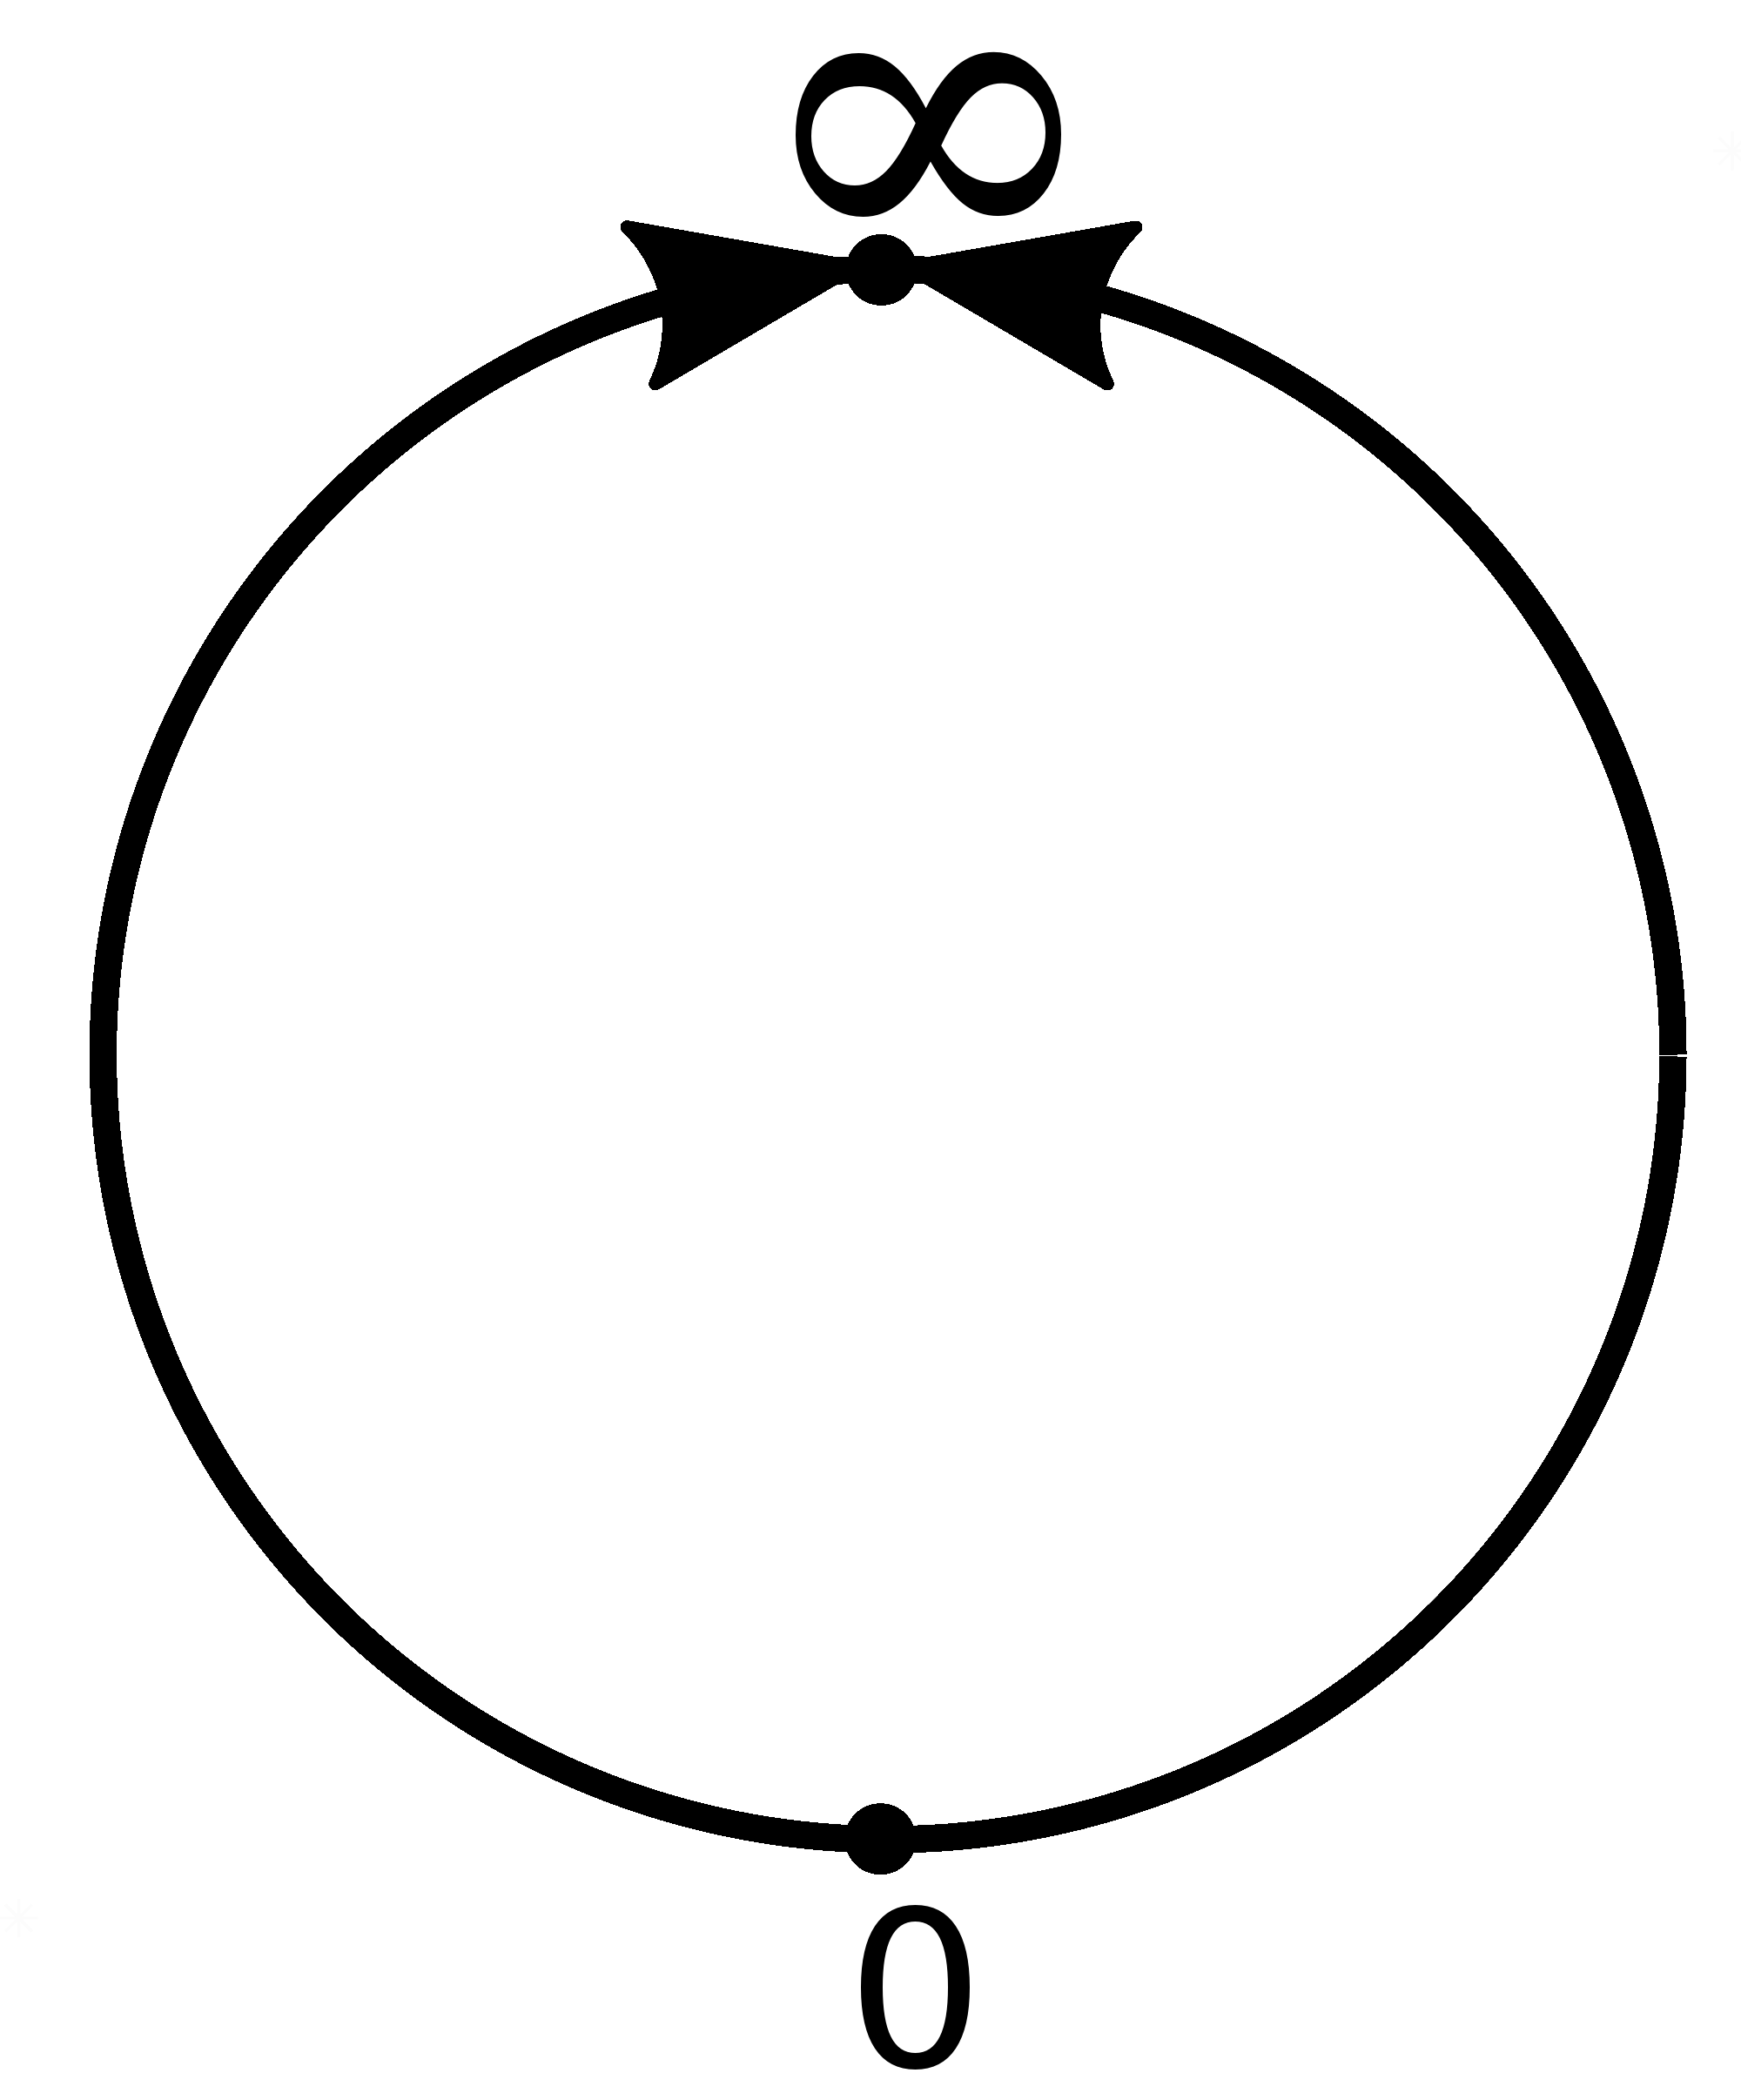
\includegraphics[width=0.38\linewidth,keepaspectratio]{Real_projective_line.png}
\end{center}

Свака цијела функција, која није полином, има у тачки $\infty$ есенцијални сингуларитет. Према великој Пикардовој теореми, таква неконстатна функција, узима у произвољној шупљој околини тачке $\infty$ све вриједности из $C$, осим можда једне, и то бесконачно много пута. Ако функција $f(z)$ није цијела, али је аналитичка у шупљој околини тачке $z_0$, према теореми Сохоцког-Вајерштраса за свако $\omega\in C\bigcup\{\infty\}$ постоји $z_n\to z_0$ такав да $f(z_n)\to\omega$ када $n\to+\infty$. Функцији која има есенцијални сингуларитет у $\infty$ можемо придружити као коначан број константан дио функције.
\\Увешћемо сада дефиницију уопштене граничне вриједности.\\

\begin{definition}
Ред облика $\sum_{k=-\infty}^{+\infty}c_k(z)\cdot \frac{1}{z^k}$ или $\sum_{k=-\infty}^{+\infty}c_k(z)\cdot (z-a)^k$, чији су коефицијенти функције и $a\in C$, ћемо називати уопштеним Лорановим редом.
\end{definition}

\begin{remark}
Специјалан случај овог реда је уопштени Пјуизов\footnote{Victor Alexandre Puiseux (1820–1883)} ред. Познато је да функција има развој у Лоранов ред у тачкама у којима има отклоњив сингуларитет (ред нема главни дио), пол (главни дио реда има коначно много чланова) или есенцијални сингуларитет (главни дио реда има бесконачно много чланова).  Функција у тачкама гранања нема развој у Лоранов ред али има развој у уопштени Пјуизов ред. Ако је у питању алгебарска тачка гранања функције, онда функција у тој тачки има развој у уопштени Пјуизов ред, при чему главни дио реда има коначно много чланова. А ако је у питању трансцедентална тачка гранања функције, онда функција у тој тачки има развој у уопштени Пјуизов ред, при чему главни дио реда може да има бесконачно много чланова. Функција у трансцедентној тачки гранања има есенцијални сингуларитет.
\end{remark}

\begin{definition}
Нека функција $f(z)$ има пол у тачки $\infty$. Уопштену граничну вриједност функције $f(z)$ у тачки $\infty$, по радијалној правој $l_\alpha=\{r\cdot e^{i\alpha}|r\in R\}$, означаваћемо са $\lim^D_{z\to\infty(\alpha)}f(z)$. Лијеву и десну уопштену граничну вриједност функције $f(z)$  као и уопштену граничну вриједност у тачки $\infty$, по радијалној правој $l_\alpha$, дефинишемо на сљедећи начин: $$\lim^D_{z\to\infty(\alpha)^+}f(z)=\lim^D_{z\to+e^{i\alpha}\infty}f(z)=\lim^D_{r\to+\infty}f(r\cdot e^{i\alpha}),$$ $$\lim^D_{z\to\infty(\alpha)^-}f(z)=\lim^D_{z\to-e^{i\alpha}\infty}f(z)=\lim^D_{r\to-\infty}f(r\cdot e^{i\alpha}),$$
$$\lim^D_{z\to\infty(\alpha)}f(z)=\lim^D_{r\to\infty(0)}f(r\cdot e^{i\alpha}),$$
$$\lim^D_{z\to\infty(\alpha)}f(z)=\frac{1}{2}(\lim^D_{z\to\infty(\alpha)^+}f(z)+\lim^D_{z\to\infty(\alpha)^-}f(z)).$$
Уопштену граничну вриједност функције $f(z)$ у тачки $\infty$, која има пол у тој тачки, дефинишемо као средњу вриједност уопштених граничних вриједности по радијалним правама $\lim^D_{z\to\infty(\alpha)}f(z)$, $\alpha\in[0,2\pi)$, у ознаци $\lim^D_{z\to\infty}f(z)$.\\
Специјално, за $\alpha=0$ ($l_0=R$) важи да је: $$\lim^D_{x\to\infty(0)^+}f(x)=\lim^D_{x\to+\infty}f(x),$$ $$\lim^D_{x\to\infty(0)^-}f(x)=\lim^D_{x\to-\infty}f(x).$$
\end{definition}

\begin{definition}
Нека функција $f(z)$ има пол у тачки $a\in C$. Уопштену граничну вриједност функције $f(z)$ у тачки $a$, по радијалној правој $l_{\alpha,a}=\{a+r\cdot e^{i\alpha}|r\in R\}$, означаваћемо са $\lim^D_{z\to a(\alpha)}f(z)$. Лијеву и десну уопштену граничну вриједност функције $f(z)$ као и уопштену граничну вриједност у тачки $a$, по радијалној правој $l_{\alpha,a}$, дефинишемо на сљедећи начин: $$\lim^D_{z\to a(\alpha)^+}f(z)=\lim^D_{z\to a+e^{i\alpha}0}f(z)=\lim^D_{r\to 0^+}f(a+r\cdot e^{i\alpha}),$$ $$\lim^D_{z\to a(\alpha)^-}f(z)=\lim^D_{z\to a-e^{i\alpha}0}f(z)=\lim^D_{r\to 0^-}f(a+r\cdot e^{i\alpha}),$$
 $$\lim^D_{z\to a(\alpha)}f(z)=\lim^D_{r\to 0(0)}f(a+r\cdot e^{i\alpha}),$$
 $$\lim^D_{z\to a(\alpha)}f(z)=\frac{1}{2}(\lim^D_{z\to a(\alpha)^+}f(z)+\lim^D_{z\to a(\alpha)^-}f(z)).$$
Уопштену граничну вриједност функције $f(z)$ у тачки $a$, која има пол у тој тачки, дефинишемо као средњу вриједност уопштених граничних вриједности по радијалним правама $\lim^D_{z\to a(\alpha)}f(z)$, $\alpha\in[0,2\pi)$, у ознаци $\lim^D_{z\to a}f(z)$.\\
Специјално, за $\alpha=0$ ($l_0=R$) важи да је: $$\lim^D_{x\to a(0)^+}f(x)=\lim^D_{x\to a^+}f(x),$$ $$\lim^D_{x\to a(0)^-}f(x)=\lim^D_{x\to a^-}f(x).$$
\end{definition}

\begin{definition}
Нека је $f(z)$ функција која има отклоњив сингуларитет у тачки $a\in C\bigcup\{\infty\}$. 
Тада њену уопштену граничну вриједност рачунамо по сљедећој формули: $$\lim^D_{z\to a} f(z)=\lim^D_{z\to a(\alpha)^\pm} f(z)=\lim_{z\to a} f(z),\ \alpha\in[0,2\pi).$$ Уопштену граничну вриједност функције $f(z)=z^n\ (n\in N)$ када $z\to\infty(0)$, рачунамо по сљедећим формулама: $$\lim^D_{z\to+\infty} z^n=\int_{-1}^0 z^n dz,$$ $$\lim^D_{z\to-\infty} z^n=\int_0^1 z^n dz.$$ Уопштену граничну вриједност функције $f(z)=z^{-n}\ (n\in N)$ када $z\to 0(0)$, рачунамо по сљедећим формулама:  $$\lim^D_{z\to 0^+} z^{-n}=\int_{-\infty}^{-1} z^{-n-2} dz,$$ $$\lim^D_{z\to 0^-} z^{-n}=\int_1^{+\infty} z^{-n-2} dz.$$ Ако функција $f(z)$ нема пол у тачки $a\in C\bigcup\{\infty\}$, а лијева или десна уопштена гранична вриједност по некој од радијалних правих није коначна или не постоји, за одговарајућу уопштену граничну вриједност, као и саму уопштену граничну вриједност, узимамо константан члан развоја функције у уопштени Лоранов ред у околини тачке $a$, ако постоји и његов главни дио има коначно много чланова. У супротном, сматраћемо $c_0(z)=f(z)$ развојем функције у уопштени Лоранов ред у околини тачке $a$. Константан члан налазимо као рјешење једначине $\int d(c_0(z))=c_0(z)$. \\ 
Нека су $f(z)$ и $g(z)$ функције, које имају пол или отклоњив сингуларитет у тачки $a\in C\bigcup\{\infty\}$, и нека је $c\in C$ константа. Важе сљедеће особине: $$\lim^D_{z\to a(\alpha)^\pm}(f(z)+g(z))=\lim^D_{z\to a(\alpha)^\pm}f(z)+\lim^D_{z\to a(\alpha)^\pm}g(z),$$
$$\lim^D_{z\to a(\alpha)^\pm}(c\cdot f(z))=c\cdot\lim^D_{z\to a(\alpha)^\pm}f(z).$$
\end{definition}

\begin{example}
функције $e^x$, $\sin(x)$, $\cos(x)$ су цијеле функције. Познато је да свака цијела функција која није полином има есенцијални сингуларитет у $\infty$. \\
$\lim_{x\to+\infty}e^x=+\infty$, док граничне вриједности $\lim_{x\to+\infty}\sin(x)$ и $\lim_{x\to+\infty}\cos(x)$ не постоје. Одговарајући развоји у уопштени Лоранов ред у околини тачке $+\infty$ су: $e^x+0$, $\sin(x)+0$ и $\cos(x)+0$. Дакле, важи: $\lim^D_{x\to+\infty}e^x=\lim^D_{x\to+\infty}\sin(x)=\lim^D_{x\to+\infty}\cos(x)=0$. Наведене функције имају развој у Тејлоров ред са бесконачно много чланова $\sum_{k=0}^\infty a_nx^n$ (исти развој имају и у околини тачке $0$). Такође важи: $\lim^D_{x\to+\infty}a^x=0 (a\not=0)$.
\end{example}

\begin{example}
Функција $\ln(x)$ има у $\infty$ тачку гранања и важи $\lim_{x\to+\infty}\ln(x)=+\infty$. Њен развој у уопштени Лоранов ред у околини тачке $+\infty$ је сама функција $\ln(x)+0$, тако да важи $\lim^D_{x\to+\infty}\ln(x)=0$. Такође важи: $\lim^D_{x\to+\infty}\sqrt[n]x^m=0,\ (m,n)=1$.
\end{example}

\begin{example}
Важи да је $\lim_{z\to+\infty}H_z=+\infty$.Функција $f(z)=H_z$\footnote{Хармонијски број $H_n=\sum_{k=1}^n \frac{1}{k}=\psi^{(0)}(n+1)+\gamma$} има есенцијални сингуларитет у тачки $\infty$ и сматрамо $c_0(z)=H_z$ развојем функције у уопштени Лоранов ред у околини тачке $\infty$. Одредимо сада константан члан развоја. Ријешимо једначину: $\int d(H_z) dz=H_z$. \\
$\int \frac{1}{6}(\pi ^2-6 H_z^{(2)}) dz=H_z,$\footnote{Уопштени хармонијски број $H_n^{(s)}=\sum_{k=1}^n \frac{1}{k^s}=\zeta(s)-\zeta(s,n+1)$; Хурвицова зета функција $\zeta(s,z)\equiv\sum_{k=0}^{+\infty} \frac{1}{(k+z)^s}$}\\ 
$\psi^{(0)}(z+1)+C=H_z,$\footnote{Дигама функција $\psi^{(0)}(z)=\frac{\Gamma'(z)}{\Gamma(z)}$; гама функција $\Gamma(x)=\int_{0}^{+\infty} t^{x-1}e^{-t}dt$}\\
$C=H_z-\psi^{(0)}(z+1),$\\
$C=\gamma.$\\
Дакле, важи:\\
$\lim^D_{z\to +\infty}H_z=\gamma.$
\end{example}

\begin{theorem} Нека функција $f(z)$ има пол у тачки $a\in C\bigcup \{\infty(0)\}$, нека је $f(z)=F_1(z)+F_2(z)$ развој у Лоранов ред у тачки $a$, при чему је $F_1(z)$ главни дио а $F_2(z)$ регуларни дио Лорановог реда и нека је $c_0$ константан члан у развоју. Тада важи формула: $$\lim^D_{z\to a(\alpha)^\pm}f(z)=\lim^D_{z\to a(\alpha)^\pm}F_1(z)+c_0.$$ 
\end{theorem}

\begin{proof}
Нека је $a\in C$.\\
$\lim^D_{z\to a(\alpha)^\pm}f(z)=\lim^D_{z\to a(\alpha)^\pm}(F_1(z)+F_2(z))=\lim^D_{z\to a(\alpha)^\pm}(\sum_{k=-n}^{-1} c_k\cdot(z-a)^k+\sum_{k=0}^\infty c_k\cdot(z-a)^k)=\lim^D_{z\to a(\alpha)^\pm}\sum_{k=-n}^{-1} c_k\cdot(z-a)^k+\lim_{z\to a}\sum_{k=0}^\infty c_k\cdot(z-a)^k=\lim^D_{z\to a(\alpha)^\pm}F_1(z)+c_0=\lim^D_{z\to a(\alpha)^\pm}\sum_{k=1}^{n} c_{-k}\cdot (z-a)^{-k}+c_0=\lim^D_{r\to 0(0)^\pm}\sum_{k=1}^{n} c_{-k}\cdot (a+r^{-k}e^{-i\alpha k}-a)^{-k}+c_0=\sum_{k=1}^n c_{-k}\cdot e^{-i\alpha k} \lim^D_{r\to 0(0)^\pm} r^{-k}+c_0=\sum_{k=1}^n c_{-k}\cdot e^{-i\alpha k}(\mp\int_{\mp 1}^{\mp\infty} r^{-k-2} dr)+c_0=\sum_{k=1}^n c_{-k}\cdot e^{-i\alpha k}\frac{(\pm 1)^k}{k+1}+c_0=\sum_{k=-n}^{-1} c_{k}\cdot e^{i\alpha k}\frac{(\pm 1)^k}{2(-k+1)}+c_0.$\\ 
На сличан начин доказујемо да је тврђење теореме тачно за $a=\infty$ и да важи: $\lim^D_{z\to \pm\infty}f(z)=\sum_{k=1}^{n} c_{k}\cdot e^{i\alpha k}\frac{(\pm 1)^k}{2(k+1)}+c_0$.
\end{proof}

Такође за $a\in C$ важи:\\
$\lim^D_{z\to a(\alpha)}f(z)=\frac{1}{2}(\lim^D_{z\to\infty(\alpha)^+}f(z)+\lim^D_{z\to\infty(\alpha)^-}f(z))=\frac{1}{2}(\sum_{k=-n}^{-1} c_{k}\cdot e^{i\alpha k}\frac{(+1)^k}{-k+1}+c_0+\sum_{k=-n}^{-1} c_{k}\cdot e^{i\alpha k}\frac{(-1)^k}{-k+1}+c_0)=\sum_{k=-n}^{-1} c_{k}\cdot e^{i\alpha k}\frac{1+(-1)^k}{2(-k+1)}+c_0.$\\
На сличан начин показујемо да за $a=\infty$ важи:\\ 
$\lim^D_{z\to \infty(\alpha)}f(z)=\sum_{k=1}^n c_k\cdot e^{i\alpha k}\frac{1+(-1)^k}{2(k+1)}+c_0$.\\ 
Одавде слиједи сљедеће тврђење.

\begin{corollary}
Нека функција $f(z)$ има пол првог реда у тачки $z=a\in C\bigcup \{\infty\}$ и нека је $c_0$ константан члан развоја функције $f(z)$ у Лоранов ред у околини тачке $a$. Тада важи да је: $$\lim^D_{z\to a(\alpha)}f(z)=c_0.$$
\end{corollary}

\begin{example}
Познато је да Риманова зета функција $\zeta(z)$ има пол у $z=1$. Погледајмо сада њен развој у Лоранов ред у околини тачке $z=1$:\\
$\frac{1}{z-1}+\gamma-\gamma _1 (z-1)+\frac{1}{2} \gamma _2(z-1)^2-\frac{1}{6} \gamma _3 (z-1)^3+\frac{1}{24} \gamma _4 (z-1)^4+O((z-1)^5).$\\
Даље имамо да важи:\\ 
$\lim^D_{z\to 1(0)}\zeta(z)=\lim^D_{z\to 1(0)}(F_1(z)+c_0)=\lim^D_{z\to 1(0)}(\frac{1}{z-1}+\gamma)=0+\gamma=\gamma.$
\end{example}

\begin{theorem}
Нека функција $f(x)$ има пол у тачки $a\in C\bigcup \{\infty\}$, нека је $f(x)=F_1(x)+F_2(x)$ развој у Лоранов ред у околини тачке $a$ и нека је $c_0$ константан члан развоја. Важи формула: $$\lim^D_{z\to a}f(z)=c_0.$$\\
\end{theorem}

\begin{proof}
Пронађимо средњу вриједност добијених уопштених граничних вриједности за $\alpha\in[0,2\pi)$.\\
Нека је $a\in C$.\\
$\lim^D_{z\to a}f(z)=\frac{1}{2\pi}\cdot\int_0^{2\pi}\lim^D_{z\to a(\alpha)}f(z)d\alpha=\frac{1}{2\pi}\cdot\int_0^{2\pi}\sum_{k=-n}^{-1} c_k \frac{1}{2}\frac{1+(-1)^k}{-k+1} e^{i\alpha k}d\alpha+c_0=\frac{1}{2\pi}\cdot\sum_{k=-n}^{-1} c_k \frac{1}{2}\frac{1+(-1)^k}{-k+1} \int_0^{2\pi}e^{i\alpha k}d\alpha+c_0=0+c_0=c_0.$\\
На сличан начин доказујемо да је тврђење теореме тачно за $a=\infty$.
\end{proof}

\begin{example}
Видјели смо да Риманова зета функција $\zeta(z)$ има пол у $z=1$ и да има развој у Лоранов ред у околини тачке $z=1$:\\
$\frac{1}{z-1}+\gamma-\gamma _1 (z-1)+\frac{1}{2} \gamma _2(z-1)^2-\frac{1}{6} \gamma _3 (z-1)^3+\frac{1}{24} \gamma _4 (z-1)^4+O((z-1)^5).$\\
Имамо да важи:\\ 
$\lim^D_{z\to 1}\zeta(z)=c_0=\gamma.$
\end{example}

\section{Сумирање неких дивергентних редова. Одређивање граничних вриједности низова њихових парцијалних сума}

\begin{exercise}{Сумирати ред (1):}
$$1-1+1-1+...+(-1)^{n-1}+...=\frac{1}{2}.$$
\end{exercise} \begin{instruction}
$s_n=\frac{1}{2}\cdot ((-1)^{n+1}+1)=\frac{1}{2}\cdot (-1)^{n+1}+\frac{1}{2}$, $s=\frac{1}{2}.$
\end{instruction}

\begin{exercise}{Сумирати ред (2):}
$$1+2+4+8+...+2^{n-1}+...=-1.$$
\end{exercise} \begin{instruction}
$s_n=2^n-1$, $s=-1.$
\end{instruction}

\begin{exercise}{Сумирати ред (3):}
$$1-2+4-8+...+(-2)^{n-1}+...=\frac{1}{3}.$$
\end{exercise} \begin{instruction}
$s_n=-\frac{1}{3}\cdot ((-2)^n-1)=-\frac{1}{3}\cdot (-2)^n+\frac{1}{3}$, $s=\frac{1}{3}.$
\end{instruction}

\begin{exercise}{Сумирати ред (4):}
$$1+a+a^2+a^3+...+a^{n-1}+...=\frac{1}{1-a}.$$
\end{exercise} \begin{instruction}
$s_n=\frac{1}{a-1}\cdot (a^n-1)=\frac{1}{a-1}\cdot a^n-\frac{1}{a-1}$, $s=\frac{1}{1-a}.$
\end{instruction}

\begin{exercise}{Сумирати ред (5):}
$$1-2+3-4+...+(-n)^{n-1}+...=\frac{1}{4}.$$
\end{exercise} \begin{instruction}
$s_n=-\frac{1}{4}\cdot ((-1)^n(2n+1)-1)=-\frac{1}{4}\cdot (-1)^n(2n+1)+\frac{1}{4}$, $s=\frac{1}{4}.$
\end{instruction}

\begin{exercise}{Сумирати ред (6):}
$$1+2+3+4+...+n+...=\frac{-1}{12}.$$
\end{exercise} \begin{instruction}
$s_n=\frac{n(n+1)}{2}$, $s=\lim^D_{n\to+\infty}\frac{n(n+1)}{2}=\int_{-1}^0\frac{n(n+1)}{2}dn=-\frac{1}{12}.$
\end{instruction}

\begin{exercise}{Сумирати ред (7):}
$$1+1+1+1+...+n^0+...=\frac{-1}{2}.$$
\end{exercise}\begin{instruction}
$s_n=n$, $s=\lim^D_{n\to+\infty}n=\int_{-1}^0ndn=-\frac{1}{2}.$
\end{instruction}

\begin{exercise}{Сумирати ред (8):}
$$2+3+4+5+...+(n+1)+...=\frac{-7}{12}.$$
\end{exercise} \begin{instruction}
$s_n=\frac{n(n+3)}{2}$, $s=\lim^D_{n\to+\infty}\frac{n(n+3)}{2}=\int_{-1}^0\frac{n(n+3)}{2}dn=-\frac{7}{12}.$
\end{instruction}

\begin{exercise}{Сумирати ред (9):}
$$0+1+2+3+...+(n-1)+...=\frac{5}{12}.$$
\end{exercise} \begin{instruction}
$s_n=\frac{n(n-1)}{2}$, $s=\lim^D_{n\to+\infty}\frac{n(n-1)}{2}=\int_{-1}^0\frac{n(n-1)}{2}dn=\frac{5}{12}.$
\end{instruction}

\begin{exercise}{Сумирати ред (10):}
$$\ln1+\ln2+\ln3+\ln4+...+\ln(n)+...=\frac{1}{2}\ln(2\pi).$$
\end{exercise} \begin{instruction}
$s_n=\ln((1)_n)$, гдје је $(1)_n=\frac{\Gamma(1+n)}{\Gamma(1)}$\footnote{Похамеров симбол $(x)_n=\frac{\Gamma(x+n)}{\Gamma(x)}=x(x+1)\cdot\cdot\cdot(x+n-1)$}. \\Погледајмо развој функције $s(n)=s_n$ у уопштени Лоранов ред у околини тачке $n=\infty$:\\
$\ln(2^{-\lfloor\frac{\arg(z+1)+\pi}{2\pi}\rfloor}\csc ^{\lfloor\frac{\arg(z+1)+\pi}{2\pi}\rfloor}(\pi(z+1))+\lfloor\frac{\arg(z+1)+\pi}{2\pi}\rfloor(i\pi z+\frac{i\pi}{2}+O((\frac{1}{z})^7))+\lfloor\frac{\arg(z)+\pi}{2\pi}\rfloor(2i\pi z+i\pi+O((\frac{1}{z})^7))+((-\ln(\frac{1}{z})-1)z+\frac{1}{2} (\ln(2\pi)-\ln(\frac{1}{z}))+\frac{1}{12z}-\frac{1}{360z^3} +\frac{1}{1260z^5}+O((\frac{1}{z})^6)))$.\\$s=\frac{1}{2}\ln(2\pi).$
\end{instruction}

\begin{exercise}{Сумирати ред (11):}
$$\ln1-\ln2+\ln3-\ln4+...+(-1)^{n-1}\ln(n)+...=-\frac{1}{2}\ln(\frac{1}{2}\pi).$$
\end{exercise} \begin{instruction}
$s_n=-\frac{1}{2}(-1)^n\ln(2)+(-1)^n\ln(\Gamma(\frac{n+1}{2}))-(-1)^n\ln(\Gamma(\frac{n+2}{2}))-\frac{1}{2}\ln(2\pi)+\ln(2)$,\\
$s=-\frac{1}{2}\ln(2\pi)+\ln(2)=-\frac{1}{2}\ln(\frac{1}{2}\pi).$
\end{instruction}

\begin{exercise}{Сумирати ред (12):}
$$\cos\theta+\cos2\theta+\cos3\theta+\cos4\theta+...+\cos (n\theta)+...=-\frac{1}{2}.$$
\end{exercise} \begin{instruction}
$s_n=\frac{1}{2}\cot(\frac{\theta}{2})\sin(n\theta)+\frac{1}{2}\cos(n\theta)-\frac{1}{2}$, $s=-\frac{1}{2}.$
\end{instruction} 

\begin{exercise}{Сумирати ред (13):}
$$\sin\theta+\sin2\theta+\sin3\theta+\sin4\theta+...+\sin (n\theta)+...=\frac{1}{2}\cot\frac{\theta}{2}.$$
\end{exercise} \begin{instruction}
$s_n=-\frac{1}{2}\cot(\frac{\theta}{2})\cos(n\theta)+\frac{1}{2}\sin(n\theta)+\frac{1}{2}\cot(\frac{\theta}{2})$, $s=\frac{1}{2}\cot\frac{\theta}{2}.$
\end{instruction}

\begin{exercise}{Сумирати ред (14):}
$$\cos\theta-\cos2\theta+\cos3\theta-\cos4\theta+...+(-1)^{n-1}\cos (n\theta)+...=\frac{1}{2}.$$
\end{exercise} \begin{instruction}
$s_n=\frac{1}{2}(\cos((\theta+\pi)(n+1))+\tan\frac{\theta}{2}\cdot \sin((\theta+\pi)(n+1))+1), s=\frac{1}{2}.$
\end{instruction}

\begin{exercise}{Сумирати ред (15):}
$$\sin\theta-\sin2\theta+\sin3\theta-\sin4\theta+...+(-1)^{n-1}\sin (n\theta)+...=\frac{1}{2}\tan\frac{\theta}{2}.$$
\end{exercise} \begin{instruction}
$s_n=\frac{1}{2}(-\tan\frac{\theta}{2}\cos((\theta+\pi)n)-\sin((\theta+\pi)n)+\tan\frac{\theta}{2})$, $s=\frac{1}{2}\tan\frac{\theta}{2}.$
\end{instruction}

\begin{exercise}{Сумирати ред (16):}
$$1^{2k}-2^{2k}+3^{2k}-4^{2k}+...+(-1)^{n-1}n^{2k}+...=0(k=1,2,3,...).$$
\end{exercise} \begin{instruction}
$s_n=2^{2 k} (-1)^{n+1} \zeta (-2 k,\frac{n+1}{2})+2^{2 k} (-1)^n \zeta (-2 k,\frac{n+2}{2})-2^{2 k+1} \zeta (-2 k)+\zeta (-2 k)$, $s=(1-2^{2k+2})\zeta (-2 k)=0.$
\end{instruction}

\begin{exercise}{Сумирати ред (17):}
$$1^{2k+1}-2^{2k+1}+3^{2k+1}-4^{2k+1}+...+(-1)^{n-1}n^{2k+1}+...=\frac{2^{2k+2}-1}{2k+2}B_{2k+2}(k=0,1,2,...).$$
\end{exercise} \begin{instruction}
$s_n=2^{2 k+1} (-1)^{n+1} \zeta (-2 k-1,\frac{n+1}{2})+2^{2 k+1} (-1)^n \zeta (-2 k-1,\frac{n+2}{2})-2^{2 k+2} \zeta (-2 k-1)+\zeta (-2 k-1)$, $s=(1-2^{2k+2})\zeta (-2 k-1)=\frac{2^{2k+2}-1}{2k+2}B_{2k+2}.$ \end{instruction}

\begin{remark}
Резултати у претходне двије вјежбе слиједе из формуле (18).
\end{remark}

\begin{exercise}{Сумирати ред (18):}
$$1^k+2^k+3^k+4^k+...+n^k+...=-\frac{B_{k+1}}{k+1}(k=1,2,3,...).$$
\end{exercise} \begin{instruction}
$s_n=\frac{1}{k+1}\sum_{m=0}^k {{k+1}\choose{m}} B_m n^{k+1-m}$, при чему је $B_1=\frac{1}{2}.$\\$s=\lim^D_{n\to+\infty}(\frac{1}{k+1}\sum_{m=0}^k {{k+1}\choose{m}} B_m n^{k+1-m})=\frac{1}{k+1}\sum_{m=0}^k {{k+1}\choose{m}} B_m \lim^D_{n\to+\infty} n^{k+1-m}=\\ \frac{1}{k+1}\sum_{m=0}^k {{k+1}\choose{m}} B_m \int_{-1}^0 n^{k+1-m} dn=-\frac{1}{k+1}\sum_{m=0}^k {{k+1}\choose{m}} B_m \frac{(-1)^{k+2-m}}{k+2-m}=-\frac{1}{k+1}\cdot B_{k+1}.$
\end{instruction}

\begin{remark}
У претходној вјежби искористити чињеницу да су Бернулијеви бројеви са непарним коефицијентима већим од јединице једнаки нули и једну од сљедеће двије формуле (прва важи ако је $B_1=\frac{1}{2}$, а друга ако је $B_1=-\frac{1}{2}$): $$B_{k+1}=1-\sum_{m=0}^k {{k+1}\choose{m}} \frac{B_m}{k+2-m},$$ $$B_{k+1}=-\sum_{m=0}^k {{k+1}\choose{m}} \frac{B_m}{k+2-m}.$$
\end{remark}

\begin{exercise}{Сумирати ред (19):}
$$1^{-s}+2^{-s}+3^{-s}+4^{-s}+...+n^{-s}+...=\zeta(s)(Re(s)<1).$$
\end{exercise} \begin{instruction}
$s_n=H_n^{(s)}=\zeta(s)-\zeta(s,n+1)$, $S=\zeta(s)$.
\end{instruction}

\begin{exercise}{Сумирати ред (20):}
$$1+(-1)+0+1+(-1)+0+...=\frac{2}{3}.$$
\end{exercise} \begin{instruction}
$s_n=\lfloor \frac{2}{3}+\frac{n}{3}\rfloor-\lfloor \frac{n}{3}\rfloor$, $s=\frac{2}{3}.$
\end{instruction}

\begin{exercise}{Сумирати ред (21):}
$$1+(-1)+0+1+(-1)+0+...=\frac{1}{3}.$$
\end{exercise} \begin{instruction}
$s_n=-\lfloor -\frac{2}{3}+\frac{n}{3}\rfloor+\lfloor -\frac{1}{3}+\frac{n}{3}\rfloor$, $s=\frac{1}{3}.$
\end{instruction}

\begin{remark}
У претходне двије вјежбе смо искористили формулу (важи за $x\in R\backslash Z$) $\lfloor x\rfloor=-\frac{1}{2}+x+\frac{\sum_{k=1}^{\infty}\frac{\sin(2k\pi x)}{k}}{\pi}$.
\end{remark}

\begin{exercise}{Сумирати ред (22):}
$$1-1!+2!-3!+4!-...+(-1)^{n-1}(n-1)!+...=0,596347...$$
\end{exercise} \begin{instruction}
$s_n=-e((-1)^nE_{n+1}(1)\Gamma(n+1)+Ei(-1))\footnote{$E_n(x)=\int_{1}^{+\infty}\frac{e^{-xt}dt}{t^n}$; експоненцијални интеграл $Ei(x)=-\int_{-x}^{+\infty}\frac{e^{-t}dt}{t}$}$, $s=-eEi(-1)=0,596347...$
\end{instruction}

\begin{exercise}{Сумирати ред (23):}
$$1+1!+2!+3!+4!+...+(n-1)!+...=0,697175...$$
\end{exercise} \begin{instruction}
$s_n=(-1)^n n!!(-n-1)+!(-2)+1\footnote{Субфакторијел $!n=\frac{\Gamma(n+1,-1)}{e}$; некомплетна гама функција $\Gamma(a,x)=\int_{x}^{+\infty} t^{a-1}e^{-t}dt$}$, $s=!(-2)+1=0,697175...$
\end{instruction}

\begin{exercise}{Сумирати ред (24):}
$$1+\frac{1}{2}+\frac{1}{3}+\frac{1}{4}+\frac{1}{5}+...+\frac{1}{n}+...=\gamma=0.57721566...$$
\end{exercise} \begin{instruction}
$s_n=\ln(n)+\gamma+\varepsilon_n$, $\varepsilon_n\sim\frac{1}{2n}$; $s=\gamma.$\\
\\Такође важи: $s_n=H_n=\psi^{(0)}(n+1)+\gamma$, $s=\gamma.$
\end{instruction}

\section{Одређивање вриједности неких дивергентних интеграла}

Важе сљедеће једнакости: 

\begin{equation}
\int_0^{+\infty} \sin x dx^D= 1,
\end{equation}

\begin{equation}
\int_0^{+\infty} \ln x \sin x dx^D= -\gamma,
\end{equation}

\begin{equation}
\int_0^{+\infty} \sqrt{x} \tanh (\sqrt{x}) dx^D= -\frac{3}{4}\zeta(3).
\end{equation}

Ове и сличне једнакости су познате физичарима, нећемо их овдје доказивати. Вриједности интеграла из наведених једнакости, можемо израчунати, одређивањем уопштених граничних вриједности њима одговарајућих функција у сингуларним тачкама. И даље вриједи правило да гдје год не можемо примјенити уобичајену граничну вриједност, примјењујемо уопштену граничну вриједност.

\begin{exercise}{Одредити вриједност интеграла (25):}
$$\int_0^{+\infty} \sin x dx^D= 1.$$
\end{exercise} \begin{instruction}
$\int_0^{+\infty} \sin x dx^D=-\cos x |_0^{+\infty}=-(\lim_{x\to+\infty}^D (\cos x+0)-\cos 0)=-(0-1)=1.$ Видјети примјер 2.
\end{instruction}

\begin{exercise}{Одредити вриједност интеграла (26):}
$$\int_0^{+\infty} \ln x \sin x dx^D= -\gamma.$$
\end{exercise} \begin{instruction}
$\int_0^{+\infty} \ln x \sin x dx^D=(Ci(x)-\ln x \cos x) |_0^{+\infty}=\lim_{x\to+\infty}^D(Ci(x)-\ln x \cos x)-\lim_{x\to 0}^D(Ci(x)-\ln x \cos x)=0-\gamma=-\gamma.$\footnote{Интеграл косинуса функција $Ci(x)=-\int_x^{+\infty} \frac{\cos t dt}{t}$} \\
Погледајмо развој функције $Ci(x)-\ln x \cos x$ у уопштени Лоранов ред у околини тачке $\infty$:\\
$\cos x(\ln\frac{1}{x}+O((\frac{1}{x})^7))+\cos x(-(\frac{1}{x})^2+\frac{6}{x^4}-\frac{120}{x^6}+O((\frac{1}{x})^7))+\sin x(\frac{1}{x}-\frac{2}{x^3}+\frac{24}{x^5}+O((\frac{1}{x})^7))+O((\frac{1}{x})^9)-i\pi \lfloor \frac{1}{2}-\frac{arg(x)}{\pi}\rfloor+0.$\\
Погледајмо развој функције $Ci(x)-\ln x \cos x$ у уопштени Лоранов ред у околини тачке $0$:\\
$\gamma+\frac{1}{4}x^2(2\ln x-1)+\frac{1}{96}x^4(1-4\ln x)+\frac{x^6(6\ln x-1)}{4320}+O(x^7).$
\end{instruction}

\begin{exercise}{Одредити вриједност интеграла (27):}
$$\int_0^{+\infty} \sqrt{x} \tanh (\sqrt{x}) dx^D= -\frac{3}{4}\zeta(3).$$
\end{exercise} \begin{instruction}
$\int_0^{+\infty} \sqrt{x} h (\sqrt{x}) dx^D=(-2\sqrt{x}Li_2(-e^{-2\sqrt{x}})-Li_3(-e^{-2\sqrt{x}})+\frac{2x^\frac{3}{2}}{3}+2x\ln (e^{-2\sqrt{x}}+1)) |_0^{+\infty}=\lim_{x\to+\infty}^D(-2\sqrt{x}Li_2(-e^{-2\sqrt{x}})-Li_3(-e^{-2\sqrt{x}})+\frac{2x^\frac{3}{2}}{3}+2x\ln (e^{-2\sqrt{x}}+1)+0)-\frac{3\zeta(3)}{4}=0-\frac{3\zeta(3)}{4}=-\frac{3\zeta(3)}{4}.$\footnote{Полилогаритам функција $Li_n(z)\equiv\sum_{k=1}^{+\infty} \frac{z^k}{k^n}$}
\end{instruction}

\begin{thebibliography}{9}

\bibitem{har} G. H. Hardy, {\it Divergent series}, Oxford at the Clarendon Press (1949) 
\bibitem{ram} Bruce C. Brendt, {\it Ramanujan's Notebooks, Part 1}, Springer-Verlag New York Inc. (1985), 133-149.
\bibitem{tuc} John Tucciarone, {\it The Development of the Theory of Summable Divergent Series from 1880 to 1925}, Archive for History of Exact Sciences, Vol. 10, No. 1/2, (28.VI.1973), 1-40.

\end{thebibliography}


\end{document}